\documentclass[a4paper,12pt,french] {article}

\usepackage{../../Style}

\pagestyle{empty}

\begin{document}

\begin{center}
11/10/2021 \hfill \textbf{Interrogation - Sujet A} \hfill 1ST2S 2
\rule[4mm]{\textwidth}{1pt}
\end{center}

\vspace{-5mm}

Nom: \hfill Prénom: \hfill \

\noindent
\begin{minipage}[t]{0.54\linewidth}
\begin{exercice}
Un sac à dos est en soldes. Son étiquette indique que son prix a subi une première réduction de $50\%$, puis une deuxième de $50\%$. Son prix avant les soldes était de 60 euros.
\begin{enumerate}
\begin{comment}
\item Compléter le schéma suivant: \hfill

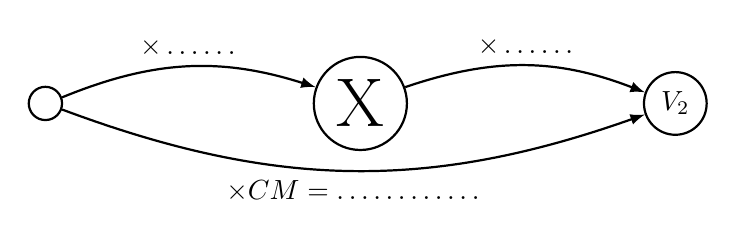
\begin{tikzpicture}
\node[draw,circle,thick] (V0) at (-4,0) {\ \hspace{1cm}};
\node[draw,circle,thick] (V1) at (0,0) {\Huge X};
\node[draw,circle,thick] (V2) at (4,0) {$V_2$};
\draw[->,>=latex,thick] (V0) to[bend left=20] node[midway,above]{$\times \ldots \ldots$} (V1);
\draw[->,>=latex,thick] (V1) to[bend left=20] node[midway,above]{$\times \ldots \ldots$} (V2);
\draw[->,>=latex,thick] (V0) to[bend right=20] node[midway,below]{$\times CM = \ldots \ldots \ldots \ldots$} (V2);
\end{tikzpicture}
\end{comment}

\item Déterminer le coefficient multiplicateur lié à la réduction globale. En déduire le taux de réduction global.

\vspace{3cm}

\item Calculer le prix soldé du sac.
\end{enumerate}

\end{exercice}
\end{minipage} % no space if you would like to put them side by side
\rule[-10.5cm]{0.5pt}{10.5cm}
\begin{minipage}[t]{0.44\linewidth}
\begin{exercice} \

\Centering{
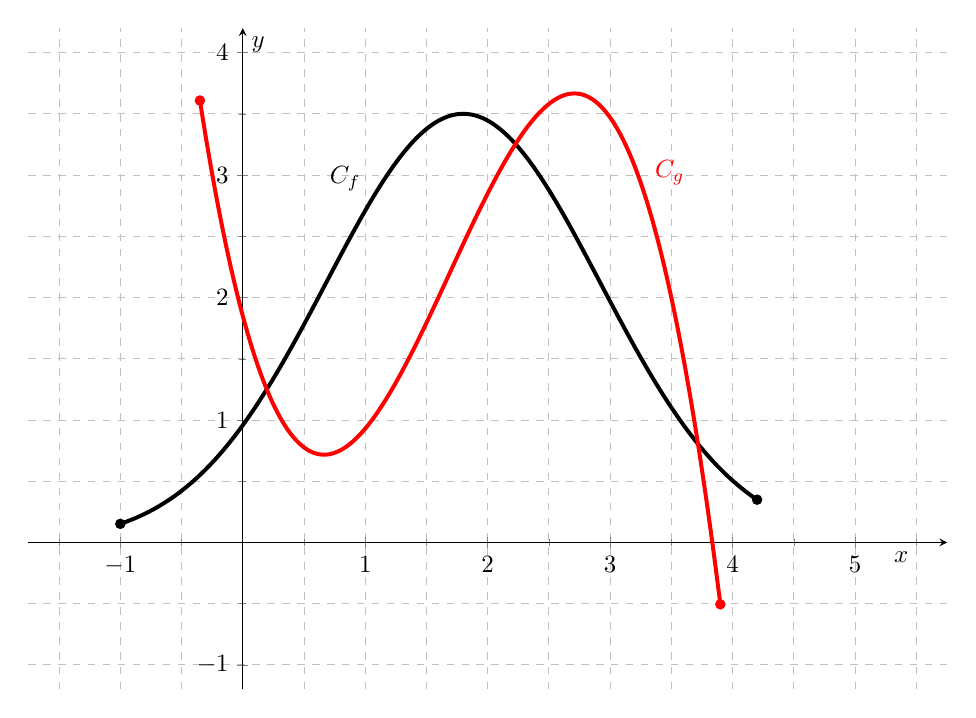
\begin{tikzpicture}[scale=0.9]
\begin{axis}[
axis x line=bottom,
axis y line = left,
axis lines=middle,
width=1.2*\linewidth,
height=0.9*\linewidth,
xmin=-0.5, xmax=4.5,
ymin=-1, ymax=4,
enlargelimits={abs=0.2},
xlabel={$x$},
ylabel={$y$},
%ytick distance=1,
minor x tick num=1,
minor y tick num=1,
axis equal,
grid=both,
grid style=dashed,
xlabel style={at={(ticklabel* cs:0.95)},below=0.1},
scale=1,
]
\addplot[samples=101,smooth,ultra thick,domain=(-1:4.2),mark=none]{3.5*e^(-0.4*(x-1.8)^2)} node [pos=0.4,above left] {$\mathscr C_f$} node[pos=0,circle, minimum size=1pt,fill,inner sep=1.5pt] {} node[pos=1,circle, minimum size=1pt,fill,inner sep=1.5pt] {};
\addplot[samples=101,smooth,ultra thick,domain=(-0.35:3.9),mark=none,color=red]{-0.69*x^3+3.49*x^2-3.72*x+1.85} node [pos=0.7,above right,color=red] {$\mathscr C_g$} node[pos=0,circle, minimum size=0pt,fill,inner sep=1.5pt] {} node[pos=1,circle, minimum size=1pt,fill,inner sep=1.5pt] {};
\end{axis}
\end{tikzpicture}}
\begin{enumerate}
\item Combien l'équation $g(x)=4$ a-t-elle de solutions?
\item Résoudre l'équation $f(x)=2$.
\vspace{15mm}
\item Résoudre l'équation $f(x)=g(x)$.
\end{enumerate}
\end{exercice}
\end{minipage}

\vfill
\setcounter{exercice}{0}

\begin{center}
11/10/2021 \hfill \textbf{Interrogation - Sujet B} \hfill 1ST2S 2
\rule[4mm]{\textwidth}{1pt}
\end{center}

\vspace{-5mm}

Nom: \hfill Prénom: \hfill \

\noindent
\begin{minipage}[t]{0.54\linewidth}
\begin{exercice}
Un sac à dos est en soldes. Son étiquette indique que son prix a subi une première réduction de $50\%$, puis une deuxième de $50\%$. Son prix avant les soldes était de 44 euros.
\begin{enumerate}
\begin{comment}
\item Compléter le schéma suivant: \hfill

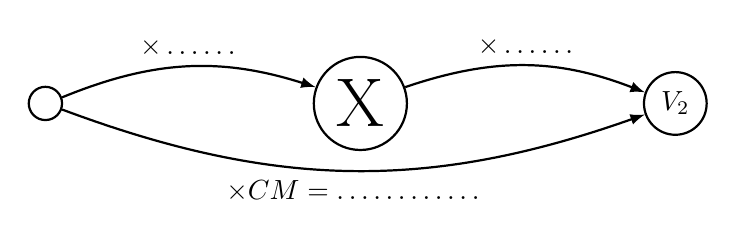
\begin{tikzpicture}
\node[draw,circle,thick] (V0) at (-4,0) {\ \hspace{1cm}};
\node[draw,circle,thick] (V1) at (0,0) {\Huge X};
\node[draw,circle,thick] (V2) at (4,0) {$V_2$};
\draw[->,>=latex,thick] (V0) to[bend left=20] node[midway,above]{$\times \ldots \ldots$} (V1);
\draw[->,>=latex,thick] (V1) to[bend left=20] node[midway,above]{$\times \ldots \ldots$} (V2);
\draw[->,>=latex,thick] (V0) to[bend right=20] node[midway,below]{$\times CM = \ldots \ldots \ldots \ldots$} (V2);
\end{tikzpicture}
\end{comment}

\item Déterminer le coefficient multiplicateur lié à la réduction globale. En déduire le taux de réduction global.

\vspace{3cm}

\item Calculer le prix soldé du sac.
\end{enumerate}

\end{exercice}
\end{minipage} % no space if you would like to put them side by side
\rule[-10.5cm]{0.5pt}{10.5cm}
\begin{minipage}[t]{0.44\linewidth}
\begin{exercice} \

\Centering{
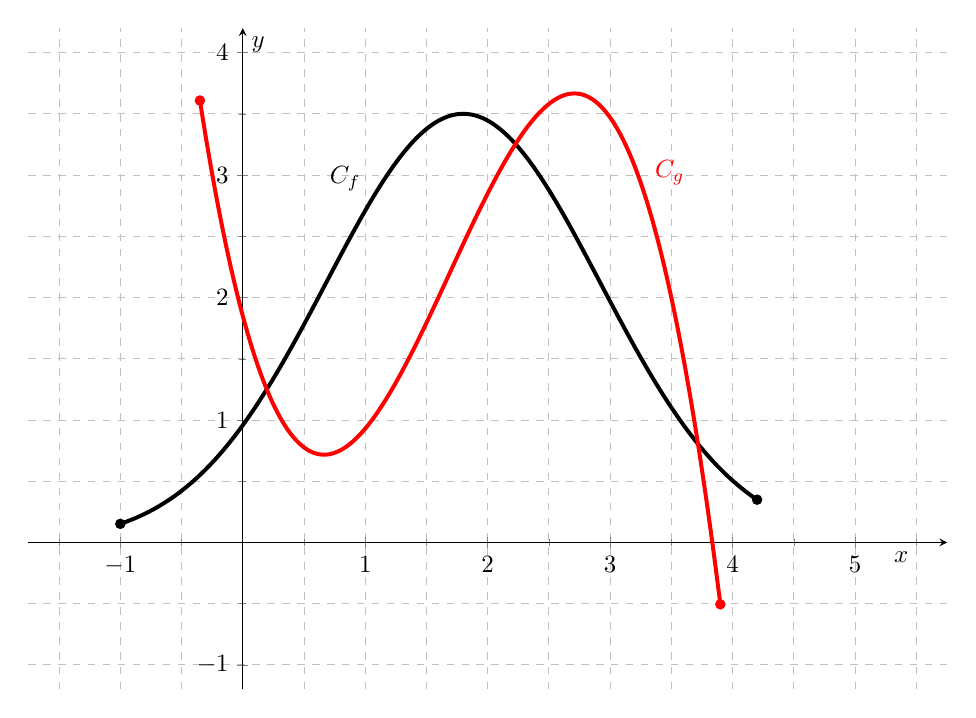
\begin{tikzpicture}[scale=0.9]
\begin{axis}[
axis x line=bottom,
axis y line = left,
axis lines=middle,
width=1.2*\linewidth,
height=0.9*\linewidth,
xmin=-0.5, xmax=4.5,
ymin=-1, ymax=4,
enlargelimits={abs=0.2},
xlabel={$x$},
ylabel={$y$},
%ytick distance=1,
minor x tick num=1,
minor y tick num=1,
axis equal,
grid=both,
grid style=dashed,
xlabel style={at={(ticklabel* cs:0.95)},below=0.1},
scale=1,
]
\addplot[samples=101,smooth,ultra thick,domain=(-1:4.2),mark=none]{3.5*e^(-0.4*(x-1.8)^2)} node [pos=0.4,above left] {$\mathscr C_f$} node[pos=0,circle, minimum size=1pt,fill,inner sep=1.5pt] {} node[pos=1,circle, minimum size=1pt,fill,inner sep=1.5pt] {};
\addplot[samples=101,smooth,ultra thick,domain=(-0.35:3.9),mark=none,color=red]{-0.69*x^3+3.49*x^2-3.72*x+1.85} node [pos=0.7,above right,color=red] {$\mathscr C_g$} node[pos=0,circle, minimum size=0pt,fill,inner sep=1.5pt] {} node[pos=1,circle, minimum size=1pt,fill,inner sep=1.5pt] {};
\end{axis}
\end{tikzpicture}}
\begin{enumerate}
\item Combien l'équation $g(x)=0$ a-t-elle de solutions?
\item Résoudre l'équation $f(x)=1$.
\vspace{15mm}
\item Résoudre l'équation $f(x)=g(x)$.
\end{enumerate}
\end{exercice}
\end{minipage}

\vfill

\end{document}
